\section*{Задачи по варианту}
\addcontentsline{toc}{section}{Задачи по варианту}




\subsection*{Задача 4. Наибольшая общая подпоследовательность двух последовательностей}
\addcontentsline{toc}{subsection}{Задача 4. Наибольшая общая подпоследовательность двух последовательностей}

Вычислить длину самой длинной общей подпоследовательности из двух
последовательностей. Даны две последовательности: $A = (a_1, a_2, ..., a_n)$ и $B = (b_1, b_2, ..., b_m)$, найти длину их самой длинной общей
подпоследовательности, т.е. наибольшее неотрицательное целое число $p$
такое, что существуют индексы $ 1 \le i_1 < i_2 < ... < i_p \le n$ и $ 1 \le j_1 < j_2 < ... < j_p \le m $ такие, что $ a_{i1} = b_{j1}, ..., a_{ip} = b_{jp}. $

\begin{itemize}
    \item Формат ввода / входного файла (input.txt).
    \newline – Первая строка: $n$ - длина первой последовательности.
    \newline – Вторая строка: $a_1, a_2, ..., a_n$ через пробел.
    \newline – Третья строка: $m$ - длина второй последовательности.
    \newline – Четвертая строка: $b_1, b_2, ..., b_m$ через пробел.
    \item Ограничения: $1 \le n, m \le 100; −10^9 < a_i, b_i < 10^9$.
    \item Формат вывода / выходного файла (output.txt). Выведите число $p$.
    \item Ограничение по времени. 1 сек.
\end{itemize}
\addcontentsline{toc}{subsubsection}{Условие задачи}

\begin{code}
	\inputminted[breaklines=true, xleftmargin=1em, linenos, frame=single, framesep=10pt, fontsize=\footnotesize, firstline=1, lastline=29]{python}{listings/task4.py}
\end{code}
\addcontentsline{toc}{subsubsection}{Листинг кода}
\newline
Длина общих подпоследовательностей хранится в двумерном списке,
каждая мера которого отвечает за одну из данных последовательностей.
Длина общей подпоследовательности для каждой ячейки списка
определяется его предыдущими ячейками.
\addcontentsline{toc}{subsubsection}{Текстовое объяснение решения}

\newpage
Результат работы кода на примерах из текста задачи:\ref{pic4}
\begin{figure}[H]
    \label{pic4}
	\begin{center}
		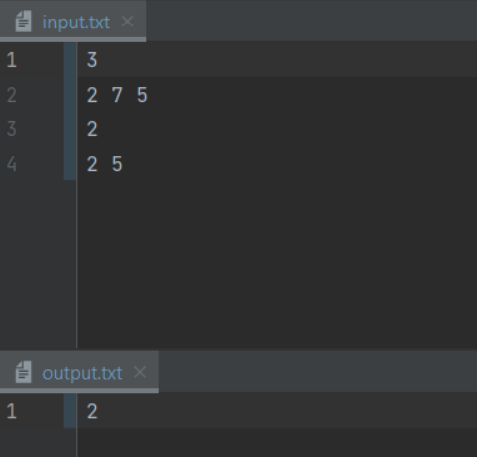
\includegraphics[scale=0.7]{fig/4_text.png}
	\end{center}
\end{figure}
\newline
Результат работы кода на минимальных и максимальных значениях:\ref{pic3}
\begin{figure}[H]
        \label{pic3}
	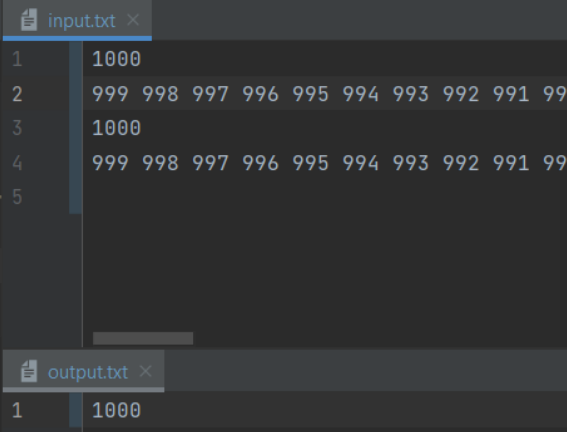
\includegraphics[scale=0.7]{fig/4_max.png}
	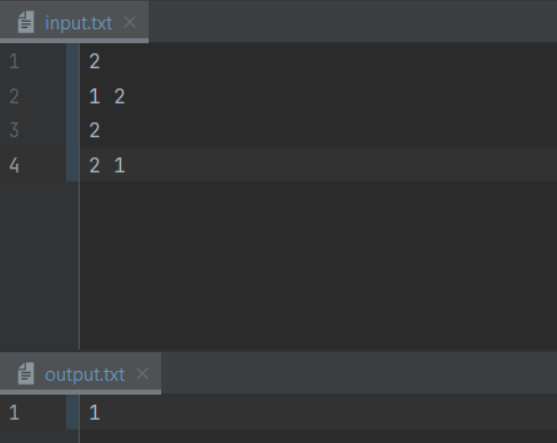
\includegraphics[scale=0.7]{fig/4_min.png}
\end{figure}
\addcontentsline{toc}{subsubsection}{Результаты работы кода}

\newpage
\begin{table}[]
    \begin{center}
        \begin{tabular}{|l|l|l|}
        \hline
             & Время выполнения & Затраты памяти  \\ \hline
            \begin{tabular}[c]{@{}l@{}}Нижняя граница\\ диапазона значений\\ входных данных из\\ текста задачи\end{tabular}  &  0.078375 seс  &  17.244140625 KB \\ \hline
            Пример из задачи  &  0.078375 sec  &  17.244140625 KB \\ \hline
            \begin{tabular}[c]{@{}l@{}}Верхняя граница\\ диапазона значений\\ входных данных из\\ текста задачи\end{tabular} & 0.078375 sec  & 17.244140625 KB \\ \hline
        \end{tabular} 
    \end{center}
\end{table}
\addcontentsline{toc}{subsubsection}{Время выполнения и затраты памяти}

\newline
\textbf{Вывод по задаче:} \newline
В задаче я реализовала алгоритм поиска длины наибольшей общей подпоследовательности для двух последовательностей.
\cite{wiki}
\addcontentsline{toc}{subsubsection}{Вывод по задаче}







\newpage
\section*{Дополнительные задачи}
\addcontentsline{toc}{section}{Дополнительные задачи}

\subsection*{Задача 5. Наибольшая общая подпоследовательность трёх последовательностей}
\addcontentsline{toc}{subsection}{Задача 5. Наибольшая общая подпоследовательность трёх последовательностей}

Вычислить длину самой длинной общей подпоследовательности из двух
последовательностей. Даны три последовательности: $A = (a_1, a_2, ..., a_n)$, $B = (b_1, b_2, ..., b_m)$ и $C = (c_1, c_2, ..., c_k)$ найти длину их самой длинной общей
подпоследовательности, т.е. наибольшее неотрицательное целое число $p$
такое, что существуют индексы $ 1 \le i_1 < i_2 < ... < i_p \le n$, $ 1 \le j_1 < j_2 < ... < j_p \le m $ и $ 1 \le k_1 < k_2 < ... < k_p \le n$ такие, что $ a_{i1} = b_{j1} = c_{k1}, ..., a_{ip} = b_{jp}  c_{kp}.

\begin{itemize}
    \item Формат ввода / входного файла (input.txt).
    \newline – Первая строка: $n$ - длина первой последовательности.
    \newline – Вторая строка: $a_1, a_2, ..., a_n$ через пробел.
    \newline – Третья строка: $m$ - длина второй последовательности.
    \newline – Четвертая строка: $b_1, b_2, ..., b_m$ через пробел.
    \newline – Пятая строка: $k$ - длина третьей последовательности.
    \newline – Шестая строка: $cс_1, c_2, ..., c_k$ через пробел.
    \item Ограничения: $1 \le n, m \le 100; −10^9 < a_i, b_i < 10^9$.
    \item Формат вывода / выходного файла (output.txt). Выведите число $p$.
    \item Ограничение по времени. 1 сек.\eqref{eq:eq1}
\end{itemize}
\addcontentsline{toc}{subsubsection}{Условие задачи}



\newline
\begin{equation}
    \centering
    \label{eq:eq1}
        y = \frac{x^2-3}{x-2}.
\end{equation}
\newpage
\begin{code}
	\inputminted[breaklines=true, xleftmargin=1em, linenos, frame=single, framesep=10pt, fontsize=\footnotesize, firstline=1, lastline=34]{python}{listings/task5.py}
\end{code}
\addcontentsline{toc}{subsubsection}{Листинг кода}
\newline
Длина общих подпоследовательностей хранится в трёхмерном списке,
каждая мера которого отвечает за одну из данных последовательностей.
Длина общей подпоследовательности для каждой ячейки списка
определяется его предыдущими ячейками. \newline
\addcontentsline{toc}{subsubsection}{Текстовое объяснение решения}

\newpage
Результат работы кода на примерах из текста задачи:\ref{pic1}
\begin{figure}[H]
        \label{pic1}
	\begin{center}
		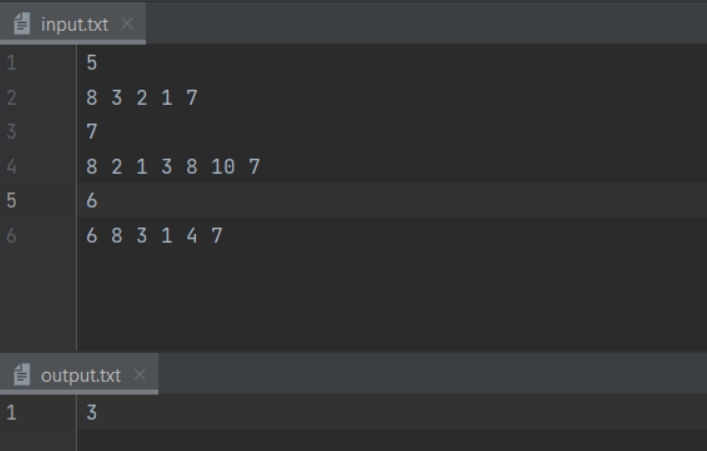
\includegraphics[scale=0.7]{fig/5_text.png}
	\end{center}
\end{figure}
\newline
Результат работы кода на минимальных и максимальных значениях:\ref{pic2}
\begin{figure}[H]
        \label{pic2}
	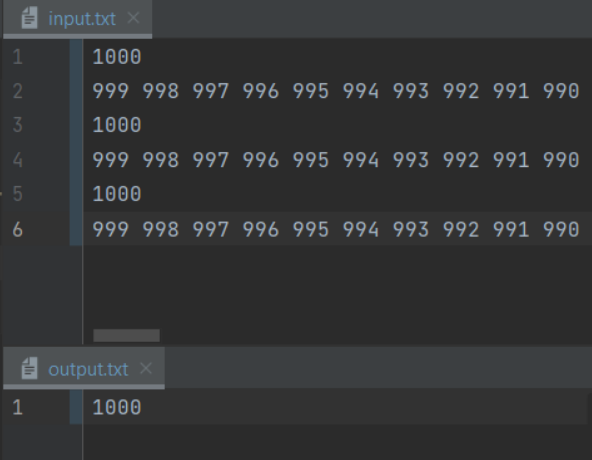
\includegraphics[scale=0.7]{fig/5_max.png}
	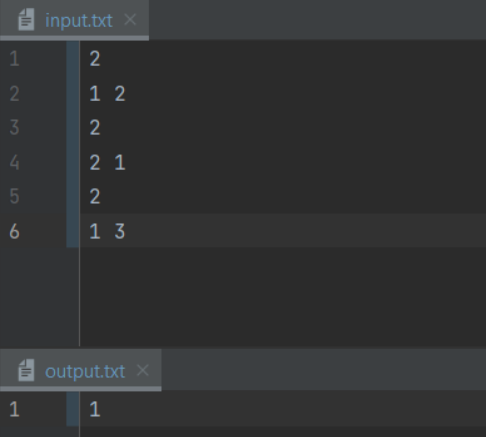
\includegraphics[scale=0.7]{fig/5_min.png}
\end{figure}
\addcontentsline{toc}{subsubsection}{Результаты работы кода}

\newpage
\begin{table}[]
    \begin{center}
        \begin{tabular}{|l|l|l|}
        \hline
             & Время выполнения & Затраты памяти  \\ \hline
            \begin{tabular}[c]{@{}l@{}}Нижняя граница\\ диапазона значений\\ входных данных из\\ текста задачи\end{tabular}  &  0.078375 seс  &  17.244140625 KB \\ \hline
            Пример из задачи  &  0.078375 sec  &  17.244140625 KB \\ \hline
            \begin{tabular}[c]{@{}l@{}}Верхняя граница\\ диапазона значений\\ входных данных из\\ текста задачи\end{tabular} & 0.078375 sec  & 17.244140625 KB \\ \hline
        \end{tabular} 
    \end{center}
\end{table}
\addcontentsline{toc}{subsubsection}{Время выполнения и затраты памяти}

\newline
\textbf{Вывод по задаче:} \newline
В задаче я реализовала алгоритм поиска длины наибольшей общей подпоследовательности для трёх последовательностей.
\addcontentsline{toc}{subsubsection}{Вывод по задаче}








\newpage
\section*{Вывод:}
\addcontentsline{toc}{section}{Вывод}
В работе я вспомнила принципы динамического программирования и их
применение к задачам про общие подпоследовательности.
\newline
\newline
